\section{Inngangur}
oijasdiojasodijasoidjaosdjoasijdasoidj
Hér skal gera lýsingu á verkefninu þ.e hvað,  hvernig og  hvaða forritunarmál, fyrir hverja og hvaða notagildi verkefnið hefur. Minnst 500 orð. Notagildi skiptir miklumáli, reynið að sjá fyrir ykkur hverjir geti notað vélmennið ykkar og í hvaða tilgangi.  Þá kemur í ljós að 500 orð er frekar lítið :-) Hér er gott að byrja á því að lesa til um Arduino en allt hjá þeim er open-sourse og svo er hægt að lesa sér til um efnið í útgefnum bókum sem "programming Arduino \cite{monk} Skoðið vel heimildaskrá og skránna mybib.bib. Hér er gott að lýsa högun kerfisins með orðum og mynd sem þið getið gert í draw.io sjá mynd: 
\begin{figure}[h]
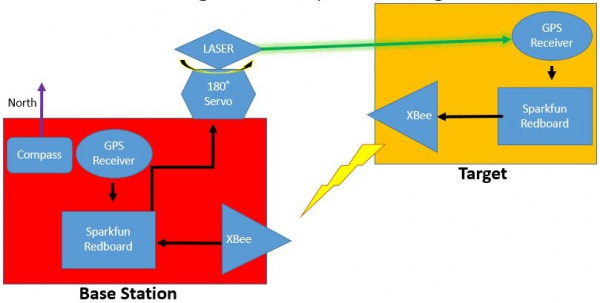
\includegraphics[scale=.3]{img/system}
\end{figure}
